%% ---------------------------------------------------------------------------
%% Joint H0 + AGN-hosted-fraction inference from dark sirens with two tracers
%%
%% Build:  python scripts/build_values.py
%%         python scripts/make_figures.py
%%         pdflatex main && bibtex main && pdflatex main && pdflatex main
%%
%% Every number in the body and the captions comes from
%% values/results_macros.tex, which scripts/build_values.py writes from the
%% dataset metadata (../data/seed100/META.json) and from the inference runs'
%% output files.  Nothing is hand-typed.  See NUMBERS.md.
%% ---------------------------------------------------------------------------
\documentclass[twocolumn]{aastex631}

\usepackage{amsmath}

\received{\today}

%% ---- editorial scaffolding (remove before submission) ---------------------
% \todo{...} marks text waiting on a result still in production.
\newcommand{\todo}[1]{{\bf [TODO: #1]}}

%% ---- notation -------------------------------------------------------------
\newcommand{\kmsmpc}{\ensuremath{{\rm km\,s^{-1}\,Mpc^{-1}}}}
\newcommand{\Hz}{\ensuremath{H_0}}
\newcommand{\fagn}{\ensuremath{f_{\rm AGN}}}
\newcommand{\nzagn}{\ensuremath{n_{0,\rm AGN}}}
\newcommand{\lognzagn}{\ensuremath{\log_{10} n_{0,\rm AGN}}}
\newcommand{\Neff}{\ensuremath{N_{\rm eff}}}
\newcommand{\Nobs}{\ensuremath{N_{\rm obs}}}
\newcommand{\Msun}{\ensuremath{M_\odot}}
\newcommand{\dd}{\ensuremath{\mathrm{d}}}

%% ---- generated values -----------------------------------------------------
% results_macros.tex -- GENERATED, DO NOT EDIT BY HAND
% written 2026-09-18T08:19:21Z by scripts/build_values.py
% 221 macros; dataset of record v3 + D3, seed 100

\newcommand{\HzeroTruth}{67.74}
\newcommand{\OmZeroTruth}{0.3075}
\newcommand{\ObZeroTruth}{0.0486}
\newcommand{\FieldZmax}{1.0}
\newcommand{\FieldShellDx}{200}
\newcommand{\FieldNshell}{16}
\newcommand{\FieldNside}{128}
\newcommand{\FieldLmax}{256}
\newcommand{\NGal}{\ensuremath{10^{-3}}}
\newcommand{\NAgn}{\ensuremath{10^{-5}}}
\newcommand{\DensityRatioTarget}{100}
\newcommand{\BiasGal}{1.2}
\newcommand{\BiasAgn}{2.0}
\newcommand{\BiasRatio}{1.67}
\newcommand{\CatNgal}{\ensuremath{1.5\times10^{8}}}
\newcommand{\CatNagn}{\ensuremath{1.5\times10^{6}}}
\newcommand{\DensityRatio}{99.8}
\newcommand{\BiasRatioMeas}{\ensuremath{1.68 \pm 0.01}}
\newcommand{\PhiStar}{\ensuremath{1.6\times10^{-2}}}
\newcommand{\SchechterAlpha}{\ensuremath{-1.07}}
\newcommand{\MagBStar}{\ensuremath{-20.47}}
\newcommand{\LumCut}{1.09}
\newcommand{\MagBLimit}{\ensuremath{-20.56}}
\newcommand{\EvNobs}{1\,000}
\newcommand{\EvFagn}{0.30}
\newcommand{\EvNsamp}{2\,000}
\newcommand{\EvSnrThresh}{8}
\newcommand{\EvSigmaRho}{1.0}
\newcommand{\EvAmc}{0.08}
\newcommand{\EvAq}{0.60}
\newcommand{\EvAchi}{0.20}
\newcommand{\EvWidthRefSnr}{8}
\newcommand{\EvSnrRef}{6.28}
\newcommand{\EvSnrRefSky}{11.5}
\newcommand{\EvSkyCoef}{35}
\newcommand{\EvSkyMin}{1}
\newcommand{\EvSkyMax}{12}
\newcommand{\EvSkyRhoScale}{1.832}
\newcommand{\EvSkyCoefEff}{19.1}
\newcommand{\EvSigmaLnDlCoef}{1.133}
\newcommand{\EvSigmaLnDlThresh}{14.2}
\newcommand{\PopAlpha}{2.3}
\newcommand{\PopMmin}{5}
\newcommand{\PopMmax}{80}
\newcommand{\PopDmMin}{3}
\newcommand{\PopDmMax}{10}
\newcommand{\PopPeakFrac}{0.90}
\newcommand{\PopPeakMu}{35}
\newcommand{\PopPeakSigma}{5}
\newcommand{\PopBeta}{1}
\newcommand{\PopChiSigma}{0.10}
\newcommand{\PopGamma}{0}
\newcommand{\EvFagnReal}{0.295}
\newcommand{\EvNhostGal}{705}
\newcommand{\EvNhostAgn}{295}
\newcommand{\EvNuniqueAgn}{294}
\newcommand{\EvMaxPerAgn}{2}
\newcommand{\EvHorizonZ}{0.31}
\newcommand{\EvZmedian}{0.13}
\newcommand{\EvNproposed}{200\,000}
\newcommand{\EvNdetTotal}{1\,570}
\newcommand{\EvDetFrac}{0.785}
\newcommand{\EvMalmquist}{18}
\newcommand{\EvSnrMedian}{10.03}
\newcommand{\EvSnrMax}{240.3}
\newcommand{\EvSigLnMcMedian}{0.0638}
\newcommand{\EvSigLnQMedian}{0.478}
\newcommand{\EvSigChiMedian}{0.159}
\newcommand{\EvSigmaLnDlMedian}{0.1137}
\newcommand{\EvSkyMinReal}{1.00}
\newcommand{\EvSkyMaxReal}{2.39}
\newcommand{\SurveyNside}{32}
\newcommand{\SurveyNpix}{12\,288}
\newcommand{\CatDzScale}{\ensuremath{3.0\times10^{-3}}}
\newcommand{\CatPhotozPullSd}{1.0000}
\newcommand{\CatPhotozPullSdAgn}{0.9996}
\newcommand{\MagLimDeep}{21}
\newcommand{\MagLimShallow}{18}
\newcommand{\MagLimStep}{1}
\newcommand{\MagLimN}{4}
\newcommand{\CompMTwentyOne}{100}
\newcommand{\CompAgnMTwentyOne}{100}
\newcommand{\CompMTwenty}{81}
\newcommand{\CompAgnMTwenty}{81}
\newcommand{\CompMNineteen}{32}
\newcommand{\CompAgnMNineteen}{32}
\newcommand{\CompMEighteen}{10}
\newcommand{\CompAgnMEighteen}{10}
\newcommand{\CompAgnMaxDev}{0.2}
\newcommand{\AgnEmptyPix}{0}
\newcommand{\AgnEmptyPixShallow}{53}
\newcommand{\AgnPerPix}{178}
\newcommand{\InjNdrawMain}{\ensuremath{1.5\times10^{8}}}
\newcommand{\InjNdrawCross}{\ensuremath{4.0\times10^{8}}}
\newcommand{\InjNdetMain}{2\,205\,380}
\newcommand{\InjNdetCross}{1\,230\,471}
\newcommand{\InjWeightPop}{0.65}
\newcommand{\InjWeightUni}{0.10}
\newcommand{\InjWeightAgn}{0.25}
\newcommand{\NeffFactor}{5}
\newcommand{\NeffMin}{\ensuremath{2.3\times10^{5}}}
\newcommand{\HzeroScanLo}{50}
\newcommand{\HzeroScanHi}{100}
\newcommand{\PeZmax}{0.65}
\newcommand{\KdePeRatio}{4.1}
\newcommand{\KdeWindow}{4\,096}
\newcommand{\HzeroGal}{\ensuremath{69.9^{+1.7}_{-1.6}}}
\newcommand{\HzeroGalMedian}{69.9}
\newcommand{\HzeroGalNinety}{\ensuremath{69.9^{+3.0}_{-2.7}}}
\newcommand{\HzeroGalWidth}{3.30}
\newcommand{\HzeroGalCross}{70.0}
\newcommand{\HzeroAgnRailMedian}{99.8}
\newcommand{\HzeroAgnRailCross}{99.8}
\newcommand{\HzeroJoint}{\ensuremath{69.2^{+1.0}_{-1.0}}}
\newcommand{\HzeroJointMedian}{69.2}
\newcommand{\HzeroJointWidth}{1.94}
\newcommand{\HzeroJointCross}{69.3}
\newcommand{\HzeroJointMap}{69.25}
\newcommand{\FagnJoint}{\ensuremath{0.273^{+0.049}_{-0.047}}}
\newcommand{\FagnJointMedian}{0.273}
\newcommand{\FagnJointWidth}{0.096}
\newcommand{\FagnJointCross}{0.267}
\newcommand{\FagnJointMap}{0.275}
\newcommand{\FagnTruthReal}{0.295}
\newcommand{\FagnTruthPlanted}{0.30}
\newcommand{\FagnBinomialSd}{0.014}
\newcommand{\JointRho}{0.068}
\newcommand{\JointRhoMean}{\ensuremath{+0.084 \pm 0.027}}
\newcommand{\ClosureScatterHzeroRatio}{0.84}
\newcommand{\ClosureScatterFagnRatio}{1.23}
\newcommand{\HzeroWidthRatio}{1.7}
\newcommand{\ClosureNseeds}{9}
\newcommand{\ClosureNother}{8}
\newcommand{\ClosureHzero}{\ensuremath{+0.50 \pm 0.33}}
\newcommand{\ClosureFagnReal}{\ensuremath{-0.013 \pm 0.020}}
\newcommand{\ClosureFagnPlanted}{\ensuremath{-0.018 \pm 0.021}}
\newcommand{\ClosureHzeroInSixtyEight}{5}
\newcommand{\ClosureHzeroInNinety}{8}
\newcommand{\ClosureFagnInSixtyEight}{5}
\newcommand{\ClosureFagnInNinety}{8}
\newcommand{\EnsCtrlNseeds}{91}
\newcommand{\EnsGalRatio}{1.00}
\newcommand{\EnsAgnRatio}{1.26}
\newcommand{\EnsCtrlGalOffset}{\ensuremath{+0.06 \pm 0.26}}
\newcommand{\EnsCtrlGalRatio}{0.96}
\newcommand{\EnsCtrlAgnOffset}{\ensuremath{+0.16 \pm 0.12}}
\newcommand{\EnsCtrlAgnRatio}{1.37}
\newcommand{\EnsGalZeroIn}{both the 68\% and the 90\%}
\newcommand{\EnsAgnZeroIn}{the 90\% but not the 68\%}
\newcommand{\EnsWidthRatioCorrected}{0.29}
\newcommand{\FagnRecord}{0.266}
\newcommand{\FagnRecordCi}{\ensuremath{[0.221,\, 0.313]}}
\newcommand{\FagnNull}{0.037}
\newcommand{\FagnNullCi}{\ensuremath{[0.012,\, 0.076]}}
\newcommand{\FagnNullCiNinety}{\ensuremath{[0.004,\, 0.106]}}
\newcommand{\FagnNullWidthRatio}{0.70}
\newcommand{\FagnZeroDlnL}{28.3}
\newcommand{\FagnZero}{7.5}
\newcommand{\FagnZeroNull}{0.3}
\newcommand{\FagnZeroRecord}{7.5}
\newcommand{\CtrlGalMean}{\ensuremath{+0.81 \pm 0.62}}
\newcommand{\CtrlGalInSixtyEight}{5}
\newcommand{\CtrlGalInNinety}{5}
\newcommand{\CtrlGalMedian}{69.0}
\newcommand{\CtrlAgnMean}{\ensuremath{+0.42 \pm 0.47}}
\newcommand{\CtrlAgnInSixtyEight}{3}
\newcommand{\CtrlAgnInNinety}{4}
\newcommand{\CtrlAgnMedian}{68.6}
\newcommand{\CtrlNseeds}{5}
\newcommand{\SelMcGal}{0.23}
\newcommand{\SelMcAgn}{0.09}
\newcommand{\SelMcJointLo}{0.12}
\newcommand{\SelMcJointHi}{0.54}
\newcommand{\PureNseeds}{93}
\newcommand{\PureNevents}{1\,000}
\newcommand{\PureGalHalfWidth}{2.11}
\newcommand{\PureAgnHalfWidth}{0.47}
\newcommand{\PureWidthRatio}{4.5}
\newcommand{\PureWidthRatioPerSeed}{\ensuremath{0.23 \pm 0.01}}
\newcommand{\PureGalOffset}{\ensuremath{-0.007 \pm 0.220}}
\newcommand{\PureGalInSixtyEight}{66}
\newcommand{\PureGalInNinety}{83}
\newcommand{\PureAgnOffset}{\ensuremath{+0.068 \pm 0.062}}
\newcommand{\PureAgnInSixtyEight}{47}
\newcommand{\PureAgnInNinety}{71}
\newcommand{\PureLaneMaxGal}{0.86}
\newcommand{\PureLaneMaxAgn}{1.23}
\newcommand{\PureNscans}{372}
\newcommand{\PureMultimodalGal}{4}
\newcommand{\PureMultimodalAgn}{0}
\newcommand{\PureMultimodalMaxHeight}{0.93}
\newcommand{\HzeroIncomplete}{\ensuremath{68.7^{+1.0}_{-1.1}}}
\newcommand{\FagnIncomplete}{\ensuremath{0.286^{+0.053}_{-0.052}}}
\newcommand{\FagnWidthRatio}{1.1}
\newcommand{\HzDensitySlopeShallow}{3.2}
\newcommand{\HzDensityShiftFactorTwo}{0.97}
\newcommand{\HzDensityShiftFactorTwoDeep}{0.01}
\newcommand{\FagnDensitySlope}{0.455}
\newcommand{\FagnFree}{\ensuremath{0.497^{+0.305}_{-0.312}}}
\newcommand{\FagnFreeWidthRatio}{5.9}
\newcommand{\GalDensityFree}{\ensuremath{-3.12^{+0.21}_{-0.41}}}
\newcommand{\GalDensityFreeOffsetDex}{0.12}
\newcommand{\FagnFreeWidthOfPrior}{0.91}
\newcommand{\DensityScanGalLo}{-4}
\newcommand{\DensityScanGalHi}{-1}
\newcommand{\DensityScanAgnLo}{-6}
\newcommand{\DensityScanAgnHi}{-4}
\newcommand{\NSeedsIncomplete}{3}
\newcommand{\GalAnchorOffsetMaxDex}{0.17}
\newcommand{\PixelAnchorBiasMinDex}{0.47}
\newcommand{\PixelAnchorBiasMaxDex}{1.19}
\newcommand{\PixelAnchorEdgeGapMaxDex}{0.10}
\newcommand{\SeedLnBFmin}{11.6}
\newcommand{\SeedLnBFmax}{17.7}
\newcommand{\FagnFreeOffsetMin}{0.17}
\newcommand{\FagnFreeOffsetMax}{0.21}
\newcommand{\RelCompletenessSpanDex}{1.86}
\newcommand{\FagnRelSlope}{\ensuremath{+0.005}}
\newcommand{\FagnRelSpan}{0.016}
\newcommand{\HzeroRelSpan}{0.45}
\newcommand{\HzeroRelSlope}{\ensuremath{-0.074}}


\begin{document}

\title{A dark standard siren measurement of the Hubble constant and the
AGN-hosted fraction of compact-binary mergers}

\shorttitle{Dark sirens and the AGN-hosted fraction}
\author{I.~Maga\~na Hernandez}
\affiliation{Department of Physics, Carnegie Mellon University, Pittsburgh, PA
15213, USA}

\begin{abstract}
We measure the Hubble constant \Hz\ and the fraction \fagn\ of compact-binary
mergers hosted by active galactic nuclei (AGN) jointly, from \EvNobs\ simulated
dark standard sirens and two host catalogs, galaxies and AGN, tracing one
simulated large-scale structure. Their line-of-sight redshift priors enter the
likelihood as a mixture with weight \fagn, identified by which catalog's
structure the events prefer. With the source population at
its input values and both catalogs complete, we find
$\Hz = \HzeroJoint$~\kmsmpc\ and $\fagn = \FagnJoint$: the realised hosted
fraction (\FagnTruthReal) lies inside the 68\% interval, the input expansion
rate inside the 90\%, and the \Hz\ interval is a factor of
\HzeroWidthRatio\ narrower than from the galaxy catalog alone. The fit recovers both
parameters across five realisations, and with \Hz\ held at its input value,
scrambling the event sky positions collapses \fagn\ from \FagnRecord\ to
\FagnNull: the fraction is measured from host association. Flux-limited catalogs preserve it when completeness
follows from each catalog's magnitude limit and luminosity function: with
both host densities free, the recovered galaxy density lies inside the 68\%
interval in three realisations, while completeness estimated from the
observed counts overstates it by up to \PixelAnchorBiasMaxDex~dex and is
disfavoured by \SeedLnBFmin\ to \SeedLnBFmax\ $e$-folds. A factor-of-two error in that density moves \Hz\ by
\HzDensityShiftFactorTwoDeep~\kmsmpc\ above \CompMTwenty\ per cent
completeness, by \HzDensityShiftFactorTwo\ at \CompMEighteen\ per cent. The branching ratio between AGN-assisted and field mergers is therefore
measurable from the events that measure the expansion rate, provided the AGN
density is known.
\end{abstract}

\keywords{Gravitational waves, Cosmology, Hubble constant, Active galactic
nuclei, Galaxy catalogs}

\section{Introduction}
\label{sec:intro}

The gravitational-wave signal of a compact-binary merger fixes its luminosity
distance without any rung of the astronomical distance ladder, which makes
every detection an absolute standard siren \citep{Schutz1986, HolzHughes2005}.
Converting that distance into a measurement of the expansion rate requires a
redshift, and the one merger with an identified electromagnetic counterpart,
GW170817, delivered \Hz\ to about ten per cent \citep{Abbott2017SirenH0}.
Counterparts have not repeated. Dark standard sirens supply the missing
redshift statistically instead: rather than identifying a single host, the
analysis uses the redshift distribution of all catalogued galaxies consistent
with the event's sky localisation and marginalises over which one was the host
\citep{DelPozzo2012}. Applied to the events detected so far, that method
constrains \Hz\ to a few tens of per cent without a single counterpart
\citep{Fishbach2019, Palmese2023, GWTC3Cosmo2023, GWTC4Cosmo2025}. The
motivation for pushing it harder is external: the cosmic microwave background
gives $67.4 \pm 0.5$~\kmsmpc\ \citep{Planck2018} while the Cepheid distance
ladder gives $73.0 \pm 1.0$~\kmsmpc\ \citep{Riess2022}, and a route to \Hz\
that shares systematics with neither will arbitrate between them only once it
reaches the per cent level.

The precision of a dark-siren inference is set by the host catalog as much as
by the gravitational-wave data. Two catalog properties do the work. The first
is how sharply the catalog pins the redshift of a host given the event's sky
patch, which improves with catalog density and with the amount of structure in
the redshift distribution on the scale of the localisation
\citep{Fishbach2019, Gray2020}. The second is how well the galaxies the survey
missed are accounted for, since real catalogs are flux limited and beyond some
redshift most hosts are absent
\citep{ChenFishbachHolz2018, Finke2021, Gray2022}. Both favour the densest
available catalog, and dark-siren analyses have accordingly been built on
galaxy catalogs alone \citep{Palmese2023, GWTC3Cosmo2023}.

There is a second host population the data have something to say about. Several
formation channels place a subset of binary black hole mergers in the gas-rich,
dense environments around AGN, where gas torques and migration traps harden
binaries and can assemble massive systems through repeated mergers
\citep{Bartos2017, StoneMetzgerHaiman2017, McKernan2018,
TagawaHaimanKocsis2020}. Individual candidate counterparts have made the
association plausible without establishing it
\citep{Graham2020, Gayathri2021, BomPalmese2023}. The fraction \fagn\ of
mergers supplied by that channel is the branching ratio between AGN-assisted
assembly and everything else \citep{FordMcKernan2022}. What is known about it
is known indirectly: \fagn\ is read off features of the mass and spin
distributions that the channel is expected to imprint, at a precision of a
factor of a few \citep{McKernan2018, FordMcKernan2022}.

AGN are not distributed like galaxies, and that is what makes \fagn\
measurable from the same events that measure the expansion rate. A catalog of
luminous AGN is roughly two orders of magnitude sparser in comoving number
density than a galaxy catalog reaching the same depth \citep{Ananna2022}, and
AGN sit in more massive haloes, so they are more strongly clustered, with a
larger linear bias \citep{Krumpe2010}. Both differences enter the
line-of-sight redshift prior each catalog supplies, so the two priors differ in
normalisation and in shape, the sparse one resolving individual structures
along a line of sight where the dense one is nearly smooth. The weight of the
mixture between them is therefore identifiable. Host positions have been used
to test the association from the outside, by asking whether the detected
events' localisation volumes contain more AGN of a given class than chance
allows \citep{Bartos2017NatComm, Veronesi2022, Veronesi2023}. No dark-siren
analysis, however, has carried a second host population inside its redshift
prior, where the same association becomes a parameter measured jointly with
the expansion rate rather than a hypothesis tested against it.

We measure \Hz\ and \fagn\ jointly on a simulated universe in which both are
known and in which the two catalogs carry the densities and biases the
literature reports. One clustered density field is sampled by two tracers, a
dense galaxy population and an AGN population two orders of magnitude sparser;
\EvNobs\ mergers are drawn from the two host populations in a known proportion
and observed once each, with every measurement error a function of the observed
data rather than of the source; and the same catalog is thinned by a magnitude
limit into flux-limited versions, so that the measurement can be repeated on
the catalogs a survey would deliver.

Section~\ref{sec:methods} gives the likelihood: the mixture over catalogs, the
redshift prior each catalog supplies and how its sky dependence is normalised,
the treatment of flux-limited catalogs, and the selection function.
Section~\ref{sec:data} describes the simulated universe: one clustered density
field sampled by two tracers with literature-anchored densities and biases, and
the events observed against it. Section~\ref{sec:results} reports the
measurements: \Hz\ from one catalog at a time, \Hz\ and \fagn\ jointly, each catalog on its own hosts at equal event
counts, and both parameters on flux-limited catalogs.
Section~\ref{sec:validation} tests them, by repeating the entire construction
on independent realisations of the simulated universe and by a null test that
removes the host association while changing nothing else.
Section~\ref{sec:discussion} states what the measurement establishes and what
it depends on. Uncertainties are 68\% equal-tailed credible intervals unless
stated otherwise, a value quoted as $x \pm y$ carries its standard error, and
the input cosmology is flat $\Lambda$CDM with
$\Hz = \HzeroTruth$~\kmsmpc\ and $\Omega_{m,0} = \OmZeroTruth$.

\section{Method}
\label{sec:methods}

\subsection{A mixture of catalog redshift priors}
\label{sec:methods:mixture}

We use the standard dark-siren population likelihood
\citep{ChenFishbachHolz2018, MandelFarrGair2019, Gray2020}. For event $i$ with
data $d_i$ and parameters $\Lambda$ containing the cosmology and the source
population, the single-event evidence is
\begin{equation}
  Z_i(\Lambda) = \int \dd\theta\; p(d_i \,|\, \theta)\,
                 p_{\rm pop}(m_1, m_2, \chi \,|\, \Lambda)\,
                 p(z, \hat{n} \,|\, \Lambda),
  \label{eq:zi}
\end{equation}
where $\theta$ collects source-frame masses, effective spin, redshift and sky
direction, and $p(z, \hat{n}|\Lambda)$ is the line-of-sight redshift prior
supplied by the catalog.

When more than one catalog traces the same structure, that prior becomes a
mixture,
\begin{equation}
  p(z, \hat{n} \,|\, \Lambda) = \sum_{k=1}^{K} f_k \,
      p_k(z, \hat{n} \,|\, \Lambda), \qquad \sum_k f_k = 1,
  \label{eq:mixture}
\end{equation}
with $f_k$ the fraction of mergers hosted by the population that catalog $k$
traces. We take $K = 2$, with $k = 1$ the galaxies and $k = 2$ the AGN, so
$f_2 \equiv \fagn$ and $f_1 = 1 - \fagn$. Written this way \fagn\ is a mixture
weight and nothing else: it does not enter the mass or spin distributions, and
it is identified entirely by which catalog's redshift and sky structure the
events prefer.

\subsection{The redshift prior a catalog supplies}
\label{sec:methods:prior}

Each catalog's prior is a kernel-density estimate in redshift over the
catalogued objects in the event's HEALPix pixel \citep{Gorski2005, Gray2022},
\begin{equation}
  p_k(z, \hat{n} \,|\, \Lambda) \;\propto\; g(z; \Lambda)
     \sum_{j \,\in\, k,\; \hat{n}_j = \hat{n}}
     \frac{w_j}{W_k}\,
     \frac{\mathcal{N}(z; z_j, \sigma_j)}{\zeta_j},
  \label{eq:pcat}
\end{equation}
where $z_j$, $\sigma_j$ and $w_j$ are a catalogued object's redshift, redshift
uncertainty and weight, $g(z;\Lambda)$ is the redshift weighting set by the
comoving volume element and the merger-rate evolution, and
$\zeta_j = \int \mathcal{N}(z; z_j, \sigma_j)\, g(z;\Lambda)\, \dd z$
normalises each kernel against that weighting.

The normalisation $W_k$ is what makes \fagn\ identifiable. We normalise each
catalog's sky weighting over the survey as a whole, $W_k = \sum_j w_j$ summed
over the entire catalog, rather than over the objects in each pixel separately.
The number of catalogued hosts in a pixel then survives into the likelihood, so
a pixel rich in galaxies but poor in AGN contributes weight to the first
component of Equation~(\ref{eq:mixture}) and little to the second. Under a
per-pixel normalisation every occupied pixel is rescaled to unit weight and the
sky-density contrast between the two catalogs (the difference in where and
in how strongly each traces the density field) is discarded.

The kernel widths $\sigma_j$ must stay well below the redshift resolution of
the distance measurements,
\begin{equation}
  \sigma_z^{\rm PE} \;\simeq\; \sigma_{d_L}\, d_L \left(
     \frac{\dd d_L}{\dd z} \right)^{-1},
  \label{eq:sigmazpe}
\end{equation}
or the redshift information in the likelihood comes from the overlap of a broad
prior with the distance posterior rather than from the catalogued hosts. For a
real survey this is a requirement on photometric redshifts. In the catalogs of
\S\ref{sec:data} the kernel widths are a factor \KdePeRatio\ below
$\sigma_z^{\rm PE}$ at the median detected redshift.

\subsection{Incomplete catalogs}
\label{sec:methods:completion}

A flux-limited survey stops finding hosts beyond some redshift, and the
analysis must say what is missing. We model the missing objects of each catalog
with a smooth comoving density,
\begin{equation}
  \frac{\dd N_{{\rm miss},k}}{\dd z} =
    n_{0,k}\, \frac{\dd V_c}{\dd z}\, (1+z)^{\delta_k}
    - \frac{\dd N_{{\rm obs},k}}{\dd z},
  \label{eq:miss}
\end{equation}
distributed isotropically over the sky, so the completeness is not a free
function but follows from the assumed density and the observed counts,
\begin{equation}
  C_k(z) = \frac{\dd N_{{\rm obs},k}/\dd z}
                {n_{0,k}\, (\dd V_c/\dd z)\, (1+z)^{\delta_k}}.
  \label{eq:completeness}
\end{equation}
Each catalog's prior is then Equation~(\ref{eq:pcat}) plus a term carrying
$\dd N_{{\rm miss},k}/\dd z$ spread uniformly over the sky, and the mixture of
Equation~(\ref{eq:mixture}) runs over those completed priors. Setting
$n_{0,k} \rightarrow 0$ removes the missing budget and recovers the
complete-catalog case.

This is the mechanism by which a shallow survey still constrains \fagn: as
catalogued hosts disappear each prior migrates from its own kernel-density
estimate onto its own smooth density, and the two smooth densities still differ
by the number-density ratio. The pair $(n_{0,k}, \delta_k)$ therefore fixes how
much of each population the analysis believes it cannot see, and \nzagn\ is the
one that matters: because \fagn\ is a weight between the two priors, an error
in \nzagn\ moves the AGN prior's out-of-catalog mass and \fagn\ follows. In
the analyses of this paper the catalogs are complete and the missing budget is
switched off; the flux-limited analyses of \S\ref{sec:results:incomplete}
anchor $(n_{0,k}, \delta_k)$ at the simulation's own comoving densities.

\subsection{The selection function}
\label{sec:methods:selection}

Over $\Nobs$ detected events the likelihood is
\begin{equation}
  \ln \mathcal{L}(\Lambda) = \sum_{i=1}^{\Nobs} \ln Z_i(\Lambda)
      - \Nobs \ln \mu(\Lambda),
  \label{eq:like}
\end{equation}
with
\begin{equation}
  \mu(\Lambda) = \int \dd\theta\; P_{\rm det}(\theta)\, p(\theta \,|\, \Lambda)
  \label{eq:mu}
\end{equation}
the detectable fraction \citep{MandelFarrGair2019, Vitale2022}. Because
Equation~(\ref{eq:zi}) is a density over the observed data, $P_{\rm det}$ must
be a property of the observed data as well; \S\ref{sec:data:events} constructs
the simulated detection rule that way.

We estimate $\mu$ by importance sampling a set of simulated signal injections
stored in the cosmology-independent observables
$(m_1^{\rm det}, q, d_L)$ together with the density each was drawn from, and
require the effective sample size of that Monte Carlo estimate to satisfy
$\Neff > \NeffFactor\,\Nobs$ \citep{Farr2019}. Values of $\Lambda$ that fail
the criterion are not quoted.

Because $\mu$ is conditioned on the catalogs through Equation~(\ref{eq:pcat}),
an injection contributes only if its redshift falls within a few $\sigma_j$ of
a catalogued object in its own pixel. Injections drawn from the source
population almost never land on the sparse catalog, so at large \fagn\ the
estimate of $\mu$ is dominated by a handful of samples and the recovered
distance scale tilts. We therefore draw injections from a three-component
mixture: from the source population, from a distribution uniform in comoving
volume, and from a component placed on the catalogued AGN themselves. Each
injection stores the exact mixture density at its own coordinates, so the
estimate of Equation~(\ref{eq:mu}) remains valid for any component weights. The
third component reads the pixelated catalog file the likelihood conditions on,
so its proposal and the target cannot disagree through a pixelisation or
kernel-width mismatch. The injection sets are drawn once, against the
complete catalogs, and reused at every survey depth; the
effective-sample-size criterion is enforced at every depth.

\subsection{Evaluating the likelihood}
\label{sec:methods:inference}

At most two parameters are free at a time, so we evaluate
Equation~(\ref{eq:like}) on a grid rather than sampling it. Priors are flat, and
we quote medians with equal-tailed 68\% intervals; where the maximum lies on a
boundary of the scanned range we quote no interval. $\Omega_{m,0}$ is fixed at
\OmZeroTruth\ and the mass and spin distributions are held at their input
values, so the mass distribution is informative but not free. The free
parameters are \Hz, scanned over
$[\HzeroScanLo, \HzeroScanHi]$~\kmsmpc, and \fagn.

\section{Simulated data}
\label{sec:data}

The measurements of \S\ref{sec:results} are made on one simulated universe,
produced in three stages: a clustered two-tracer host catalog, a population of
mergers placed on that catalog and observed once each, and flux-limited
versions of the same catalog. Figure~\ref{fig:pgm} is the graph of the process.

\begin{figure*}[t]
\centering
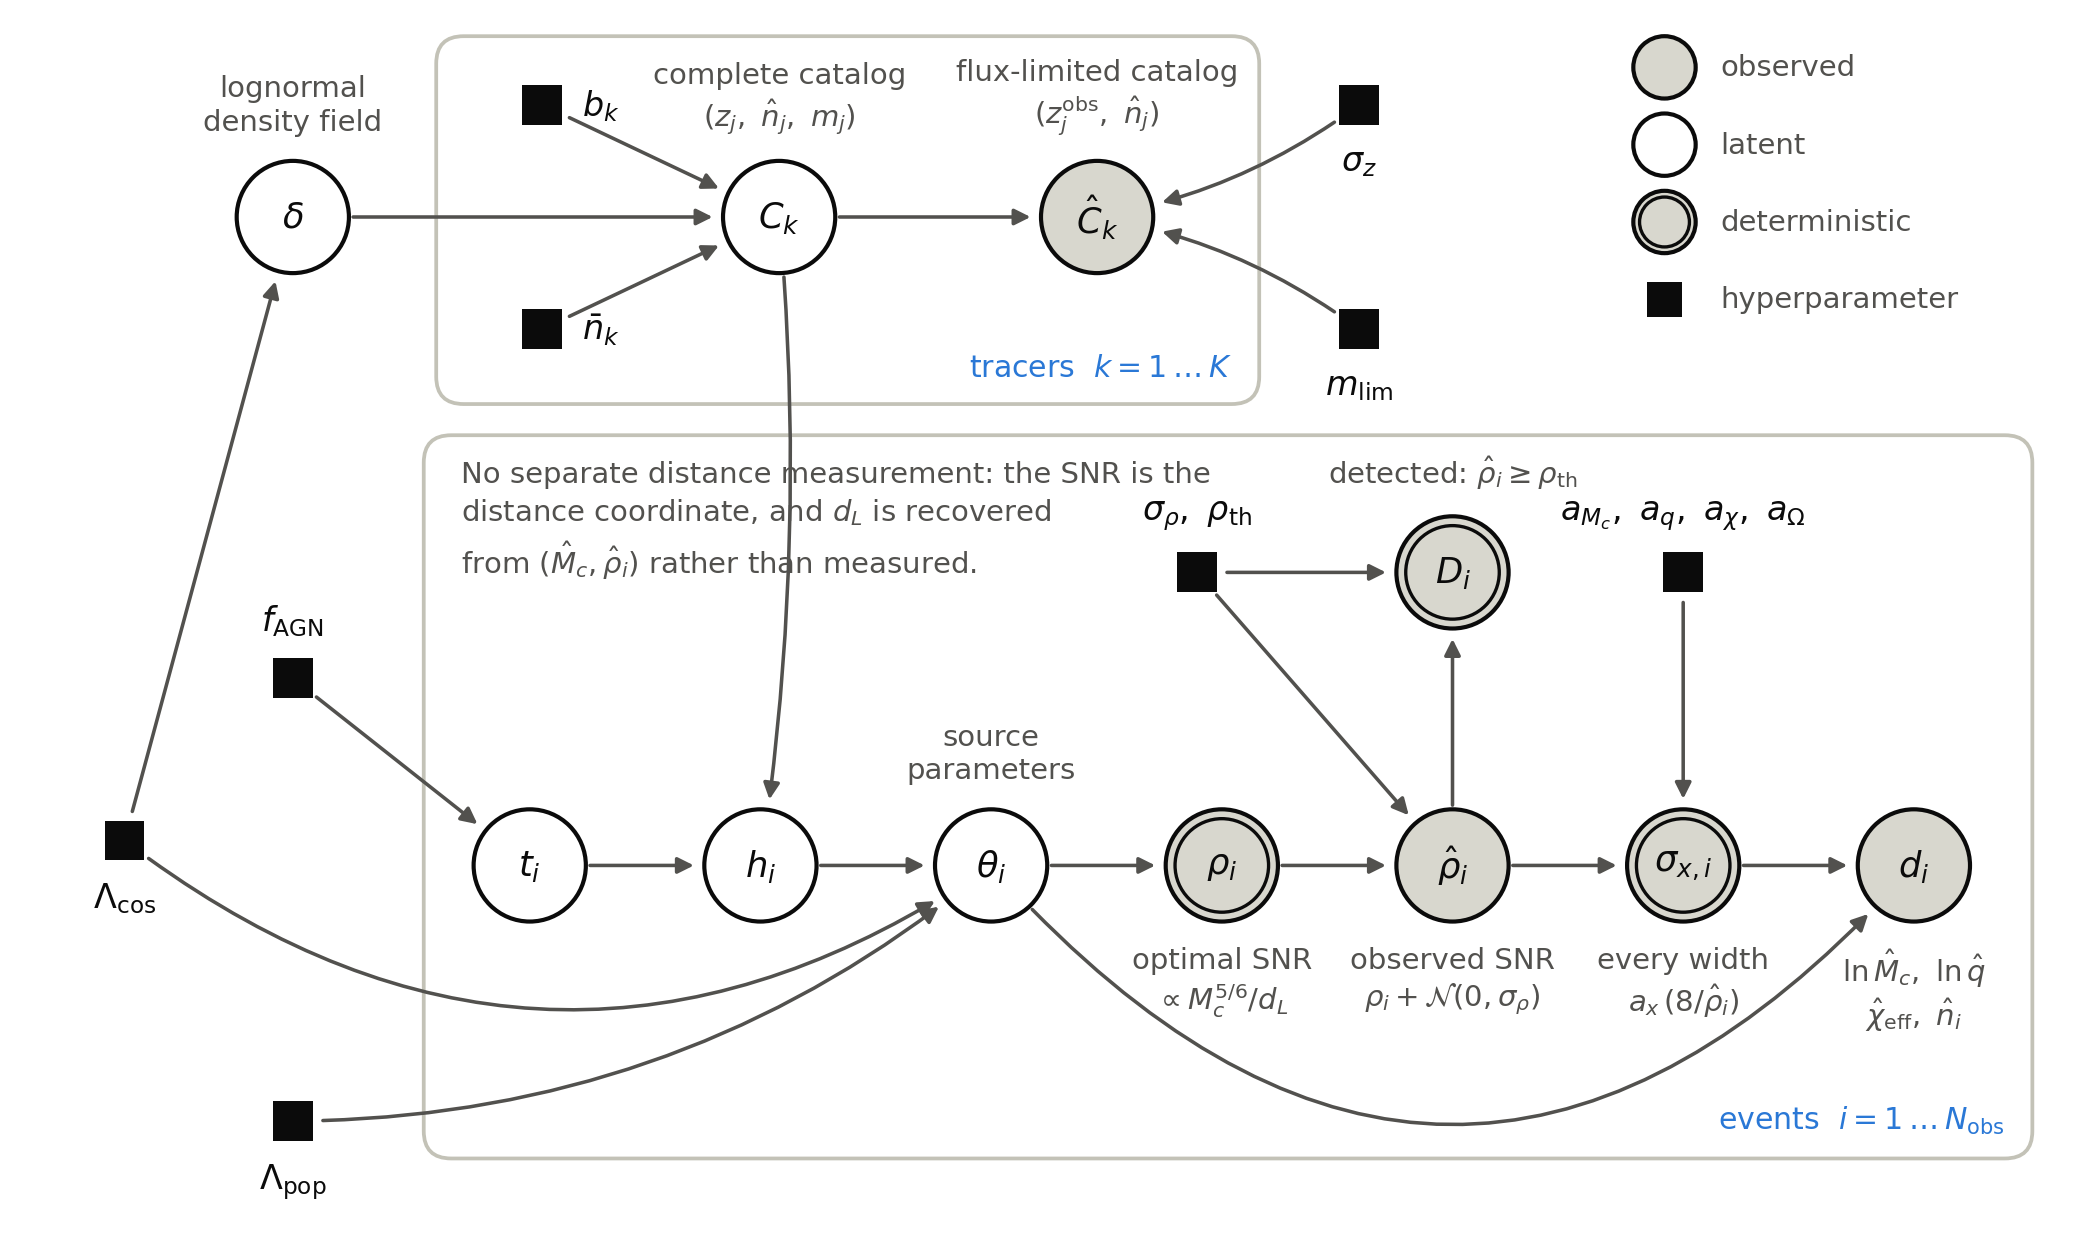
\includegraphics[width=\textwidth]{figures/fig_pgm.pdf}
\caption{The generative model of \S\ref{sec:data}. Shaded nodes are observed,
open nodes are latent, small filled squares are fixed hyperparameters, and
double-ringed nodes are deterministic functions of their parents. The cosmology
$\Lambda_{\rm cos}$ fixes the shell geometry and the matter power spectrum,
from which one lognormal density field $\delta$ is drawn. The tracer plate
($k = 1 \dots K$) samples that single field twice, each tracer with its own
linear bias $b_k$ and mean comoving density $\bar{n}_k$, into a complete
catalog $C_k$ of sky positions, photometric redshifts and magnitudes; the flux
limit $m_{\rm lim}$ thins $C_k$ into the observed catalog $\hat{C}_k$, the only
version the incomplete analyses see. The event plate ($i = 1 \dots \Nobs$)
draws a host-population label $t_i$ with probability \fagn, a host $h_i$ from
that population's \emph{complete} catalog (mergers occur whether or not a
survey catalogued the host), and source parameters $\theta_i$ from the fixed
population $\Lambda_{\rm pop}$. The source is measured once: the observed
amplitude $\rho_{{\rm obs},i}$ carries the measurement noise. Everything
downstream is a function of observed data, never of the latent source: the
detection indicator $D_i = \Theta(\rho_{{\rm obs},i} - \rho_{\rm th})$, every
measurement width, the observed direction $\hat{n}_i^{\rm obs}$, and the
derived luminosity distance. The
inference of \S\ref{sec:methods} conditions on the shaded nodes and infers
$(\Hz, \fagn)$.
\label{fig:pgm}}
\end{figure*}

\subsection{Two tracers of one density field}
\label{sec:data:field}

The background cosmology is flat $\Lambda$CDM with $\Hz = \HzeroTruth$~\kmsmpc,
$\Omega_{m,0} = \OmZeroTruth$ and $\Omega_{b,0} = \ObZeroTruth$
\citep{Planck2015}, and the nonlinear matter power spectrum is computed with
\textsc{camb} \citep{Lewis2000}. The light cone is divided into \FieldNshell\
shells of comoving thickness \FieldShellDx~Mpc out to $z = \FieldZmax$, each
with a linear radial window; projecting the matter power spectrum onto those
windows gives the shell--shell angular spectra, from which \textsc{glass}
\citep{Tessore2023} draws one realisation of a set of lognormal fields on a
HEALPix grid with $N_{\rm side} = \FieldNside$ and $\ell_{\rm max} =
\FieldLmax$. Lognormal rather than Gaussian fields matter because the sparse
tracer lives in the high-density tail.

Both tracers are sampled from that same realisation. The expected count of
tracer $k$ in pixel $p$ of shell $s$ is
\begin{equation}
  \lambda_{k,s,p} = \frac{\bar{n}_k V_{s}}{N_{\rm pix}}\,
     \max\!\left[\, 1 + b_k\, \delta_s(p),\; 0 \,\right],
  \label{eq:poisson}
\end{equation}
with $V_s$ the shell's comoving volume, and the realised count is an
independent Poisson draw; each object is placed uniformly within its pixel and
given a redshift drawn $\propto W_s(z)\,\dd V_c/\dd z$, which makes the comoving
number density constant.

The two number densities are anchored to the literature. For the galaxies we
take $\bar{n}_{\rm gal} = \NGal$~Mpc$^{-3}$, the density of the bright end of
the $B$-band Schechter function used to characterise the GLADE catalogs
($\phi^* = \PhiStar\,h^3$~Mpc$^{-3}$ with $h = 0.7$,
$\alpha = \SchechterAlpha$,
$M_B^* = \MagBStar$; \citealt{Dalya2018, Dalya2022}); on that luminosity
function the cut corresponds to $L > \LumCut\,L^*$, or
$M_B < \MagBLimit$. For the AGN we take $\bar{n}_{\rm AGN} = \NAgn$~Mpc$^{-3}$,
the space density of the luminous class $\log_{10} L_X(2$--$10\,{\rm keV})
\gtrsim 43.7$ from the integrated Swift-BAT/BASS X-ray luminosity function
\citep{Ananna2022}. The ratio of the two is \DensityRatioTarget. The linear
biases are $b_{\rm gal} = \BiasGal$ and $b_{\rm AGN} = \BiasAgn$, a contrast of
\BiasRatio.

The realised catalogs hold \CatNgal\ galaxies and \CatNagn\ AGN, with a
comoving number-density ratio of \DensityRatio. Cross-correlating the two
catalogs recovers a bias ratio of \BiasRatioMeas, within $2\sigma$ (1.1 per
cent) of the input \BiasRatio, so the clustering contrast that
Equation~(\ref{eq:mixture}) is asked to detect survives the resolution of the
field essentially undegraded.

Every object carries an absolute magnitude drawn from the same Schechter
function, converted to an apparent magnitude through the distance modulus with
no $K$-correction and no luminosity evolution. AGN inherit the luminosity
function of their host galaxies, so a single flux limit thins both catalogs
through the same completeness function and survey depth remains one axis rather
than two.

Catalogued redshifts are photometric. The observed redshift of every object is
scattered about the true one, $z_{\rm obs} = z + \mathcal{N}(0,
\epsilon_z(1+z))$ with $\epsilon_z = \CatDzScale$, the analysis sees only
$z_{\rm obs}$, and the per-object uncertainty the catalog declares matches the
scatter actually present (the normalised residuals have unit variance in both
catalogs). Mergers occur at the true redshift; the survey just does not know
it exactly.

The catalogs extend to $z = \FieldZmax$. This is a requirement rather than a
choice: the events reach $z = \EvHorizonZ$, and no posterior sample corresponds
to a redshift above $z = \PeZmax$ anywhere in the analysed range of \Hz, so the
catalogs' support extends well beyond the redshifts the gravitational-wave data
can reach and the edge of the catalog is never a lever on the inference.

\subsection{The gravitational-wave events}
\label{sec:data:events}

Events are placed on the complete catalogs, before any survey selection.

Each event is assigned a host population with probability \fagn, then a host
drawn uniformly from that population's catalog with an acceptance
$\propto (1+z)^{\gamma-1}$, so the merger redshift distribution is
$p(z) \propto (\dd V_c/\dd z)(1+z)^{\gamma-1}$ with $\gamma = \PopGamma$. The
event's redshift and sky position are its host's. Masses and effective spin are
drawn from a fixed power-law-plus-peak population independent of the host and
of the cosmology \citep{GWTC3Pop2023}, with $\alpha = \PopAlpha$,
$m_{\min} = \PopMmin\,\Msun$, $m_{\max} = \PopMmax\,\Msun$, taper widths
$\PopDmMin$ and $\PopDmMax\,\Msun$, peak weight $\PopPeakFrac$ at
$\mu = \PopPeakMu\,\Msun$ with $\sigma = \PopPeakSigma\,\Msun$, pairing index
$\beta = \PopBeta$, and $\chi \sim \mathcal{N}(0, \PopChiSigma^2)$. The input
AGN-hosted fraction is $\fagn = \EvFagn$, and events are drawn until
$\Nobs = \EvNobs$ are detected.

Each source is measured once, and that single measurement is the event. A single scalar
stands in for the network signal-to-noise ratio; its noise-free value depends
only on the detector-frame chirp mass and the luminosity distance,
\begin{equation}
  \rho_{\rm opt}\!\left(\mathcal{M}^{\rm det}, d_L\right) = \rho_{\rm ref}
     \left( \frac{\mathcal{M}^{\rm det}}{30\,\Msun} \right)^{5/6}
     \left( \frac{1\,{\rm Gpc}}{d_L} \right),
  \label{eq:snr}
\end{equation}
the inspiral scaling with the antenna response left out, with
$\rho_{\rm ref} = \EvSnrRef$ set so that the detected fraction matches a
calculation that includes the response. What is observed is this amplitude
plus its measurement noise,
$\rho_{\rm obs} = \rho_{\rm opt} + n$, $n \sim \mathcal{N}(0, \EvSigmaRho)$,
and an event is detected when $\rho_{\rm obs} \geq \EvSnrThresh$
\citep{FishbachHolzFarr2018, Farah2023}. Detection is therefore a threshold on
observed data, not on the source: Equation~(\ref{eq:zi}) is a density over the
observed data and $\mu$ normalises it over the detectable region, so the pair
is a correctly normalised density for detected events only if detection is a
property of the data themselves. \EvMalmquist\ per cent of the detected events
have a noise-free amplitude below threshold, the Malmquist scatter that only a
cut in data space produces.

Every measurement error follows the same rule: its width is a function of the
observed amplitude, never of the latent source. The detector-frame chirp mass,
mass ratio and effective spin are measured with
\begin{equation}
\begin{gathered}
  \sigma_{\ln \mathcal{M}} = \EvAmc\,\frac{\EvWidthRefSnr}{\rho_{\rm obs}},
  \qquad
  \sigma_{\ln q} = \EvAq\,\frac{\EvWidthRefSnr}{\rho_{\rm obs}},\\
  \sigma_{\chi} = \EvAchi\,\frac{\EvWidthRefSnr}{\rho_{\rm obs}},
\end{gathered}
  \label{eq:widths}
\end{equation}
the widths used to build mock catalogs for gravitational-wave population
studies \citep{FishbachHolzFarr2018, Farah2023}, and the observed sky position
is scattered about the host's with
$\sigma_{\rm ang} = \mathrm{clip}\!\left(
\EvSkyCoefEff^\circ/\rho_{\rm obs},\, \EvSkyMin^\circ,\, \EvSkyMax^\circ
\right)$, the $1/\rho$ scaling of timing triangulation \citep{Fairhurst2009};
the realised widths span \EvSkyMinReal--$\EvSkyMaxReal^\circ$. A width
computed from the true parameters instead would carry distance information
that the fixed-width posterior handed to the likelihood cannot represent.

There is no separate distance measurement. Given the observed chirp mass, the
observed amplitude fixes the distance by inverting Equation~(\ref{eq:snr}), so
the signal-to-noise ratio is the distance observable, with an effective width
$\sigma_{\ln d_L} = \EvSigmaLnDlCoef/\rho_{\rm obs}$: \EvSigmaLnDlThresh\
per cent at the detection threshold, with a median of \EvSigmaLnDlMedian\ in
$\ln d_L$ over the detected sample. Treating an independently measured
distance as a second datum alongside the amplitude would leave a
source-dependent factor in the likelihood that the inference has no parameter
for.

The event's posterior samples are exact. With flat priors on
$(\ln \mathcal{M}^{\rm det}, \ln q, \rho, \chi_{\rm eff}, \alpha, \delta)$,
the posterior conditioned on the observed values above is a product of known
one-dimensional distributions, and we draw \EvNsamp\ samples from it directly,
mapping the prior exactly into the $(m_1^{\rm det}, q, d_L, \chi_{\rm eff})$
basis the inference uses. Physical ranges ($q \leq 1$, $\rho > 0$,
$|\chi_{\rm eff}| \leq 1$) are imposed on the prior, never on the observed
values: truncating the data censors the likelihood, while truncating the
prior is exact. Sample clouds centred on the true parameters, by contrast,
would be mislabelled as flat-prior posteriors and would bias the distance
scale at order $\sigma_{\ln d_L}^2$.

The detected set contains \EvNhostGal\ galaxy-hosted and \EvNhostAgn\
AGN-hosted events, a realised fraction of \EvFagnReal\ against the input
probability of \EvFagn. It reaches $z = \EvHorizonZ$ with a median of
$z = \EvZmedian$; \EvNdetTotal\ of \EvNproposed\ proposed sources pass the
threshold (\EvDetFrac\ per cent), and the first \EvNobs\ constitute the
sample. The AGN-hosted events occupy \EvNuniqueAgn\ distinct AGN, with at most
\EvMaxPerAgn\ events sharing a host, so the sparse catalog is not carrying the
measurement through a handful of repeated hosts.

\subsection{Flux-limited catalogs}
\label{sec:data:survey}

Incomplete catalogs are produced by applying an apparent-magnitude limit
$m_j < m_{\rm lim}$ to the complete catalogs, with the same limit applied to
both tracers and the events left untouched. We use \MagLimN\ limits from
$m_{\rm lim} = \MagLimDeep$ to \MagLimShallow\ in steps of \MagLimStep\ mag.
Within the volume the events occupy, the fraction of galaxies catalogued is
\CompMTwentyOne\ per cent at the deepest limit and falls to \CompMTwenty,
\CompMNineteen\ and \CompMEighteen\ per cent at the shallower three, and the
AGN fractions differ from them by at most \CompAgnMaxDev\ percentage points.

The limit is isotropic and there is no explicit redshift cut. Both matter for
what is being measured: an anisotropic completeness modelled as isotropic by
Equation~(\ref{eq:completeness}) would imprint a sky-density contrast between
what the analysis expects and what it sees, which is the same contrast that
identifies \fagn; and letting $C_k(z)$ follow from the flux limit acting on the
luminosity function gives it the smoothly declining shape a flux-limited survey
has rather than one chosen for convenience.

The catalogs are pixelated at $N_{\rm side} = \SurveyNside$
(\SurveyNpix\ pixels) into the form Equation~(\ref{eq:pcat}) consumes, each
object entering at its observed redshift with its declared photometric
uncertainty as the kernel width, $\sigma_j = \epsilon_z(1 + z_{{\rm obs},j})$. At
this resolution the complete AGN catalog occupies every pixel, with up to
\AgnPerPix\ objects in one; at the shallowest limit \AgnEmptyPixShallow\ per
cent of pixels contain no AGN at all, and the emptiness of the sparse catalog
becomes part of the information: an AGN-hosted event cannot have come from a
pixel that holds no AGN, except through the out-of-catalog term of
\S\ref{sec:methods:completion}.

The selection function at every depth is estimated from the same
\InjNdrawMain\ injections, drawn against the complete catalogs from the
three-component mixture of \S\ref{sec:methods:selection} with weights
$\InjWeightPop$, $\InjWeightUni$ and $\InjWeightAgn$, and cross-checked
against \InjNdrawCross\ injections drawn from the population and the comoving
volume alone.

\section{Results}
\label{sec:results}

The estimator recovers the truth when it is told the truth. Handing each
catalog only the events its objects actually host returns
$\Hz = \CtrlGalMedian$~\kmsmpc\ from the galaxies (\EvNhostGal\ events) and
$\Hz = \CtrlAgnMedian$~\kmsmpc\ from the AGN (\EvNhostAgn\ events), both
consistent with the input value: it lies inside the galaxy control's
68\% interval and the AGN control's 90\%. Section~\ref{sec:validation}
repeats this recovery across five independent realisations. The measurements that
follow use all \EvNobs\ events.

\subsection{The Hubble constant from one catalog at a time}
\label{sec:results:single}

\begin{figure}[t]
\centering
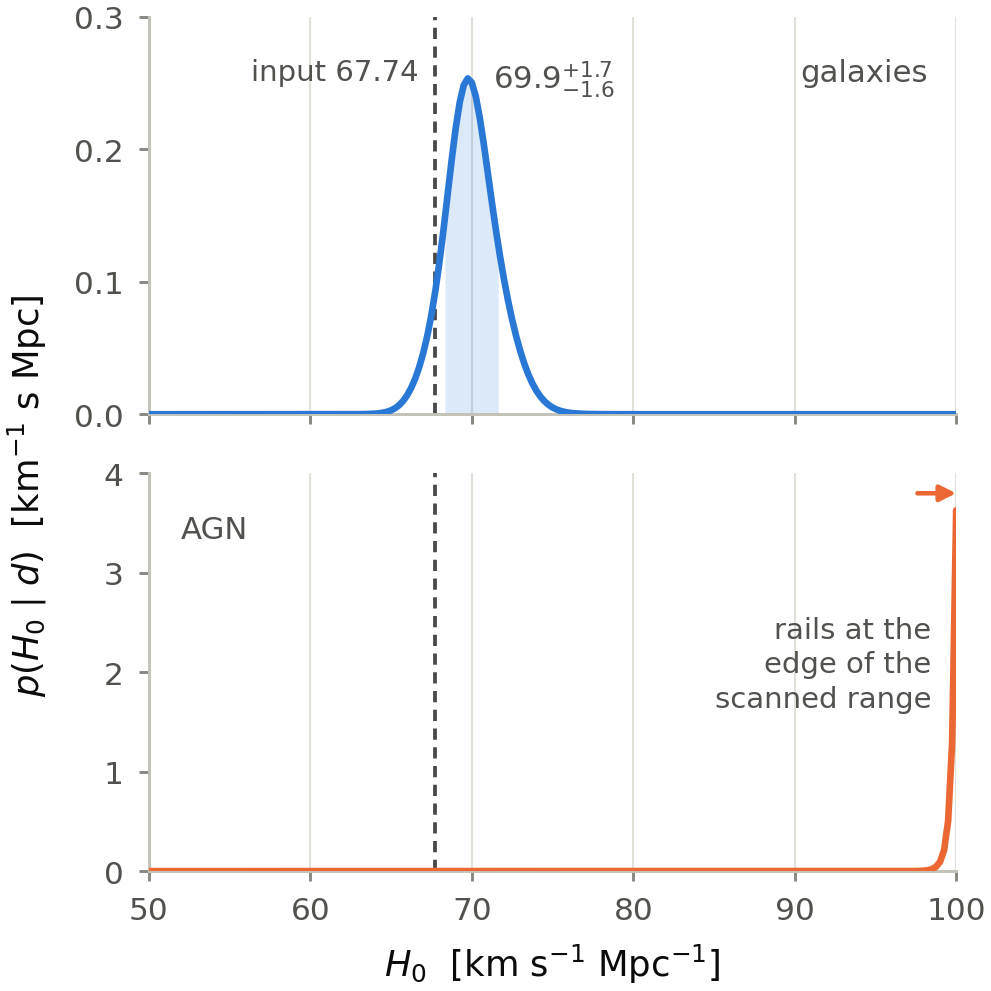
\includegraphics[width=\columnwidth]{figures/fig_single_tracer.pdf}
\caption{The same \EvNobs\ events analysed against one catalog at a time
(reference realisation, \Hz\ scanned over
$[\HzeroScanLo, \HzeroScanHi]$~\kmsmpc, the full range shown). Each panel
shows the normalised flat-prior posterior density $p(\Hz \mid d)$, in units
of km$^{-1}$\,s\,Mpc, for the galaxy catalog (top) and the AGN catalog
(bottom); the two panels share the \Hz\ axis, their density scales differ,
and no curve is rescaled. The dashed line is the input value, and the shaded
band is the galaxy analysis' 68\% interval, $\Hz = \HzeroGal$~\kmsmpc. The
AGN-only posterior has no interior maximum: it is still rising at the edge
of the scanned range, so no interval is quoted for it. Neither analysis knows
that the events were drawn from a mixture of the two catalogs.
\label{fig:single}}
\end{figure}

A single-catalog analysis asserts that every host is in that catalog, and in
this universe the assertion fails for both: the galaxy catalog is missing the
hosts of the \EvNhostAgn\ AGN-hosted events, and the AGN catalog those of the
\EvNhostGal\ galaxy-hosted ones. What differs is the price. From the galaxy
catalog alone we find $\Hz = \HzeroGal$~\kmsmpc\
(Figure~\ref{fig:single}): the input value lies within the 90\% interval but
outside the 68\%, whose full width is \HzeroGalWidth~\kmsmpc. The dense
catalog absorbs the events that do not belong to it at a modest price because
it offers many candidate hosts along every line of sight, tracing the same
structure the true hosts occupy.

The AGN catalog alone fails outright. Asked to explain \EvNobs\ events with a
catalog that hosts \EvNhostAgn\ of them, its posterior climbs into the upper
edge of the analysed range (median \HzeroAgnRailMedian\ against a boundary at
\HzeroScanHi~\kmsmpc), and we quote no interval from a posterior that peaks on
the boundary of its support. The asymmetry between the two catalogs has a
simple reading: sharp localisation cuts both ways. The sparse catalog pins its
own events to a handful of hosts, but by the same token it offers no diffuse
background of candidates that could plausibly absorb the \EvNhostGal\ events
that are not its to explain.

\subsection{The Hubble constant and the AGN-hosted fraction jointly}
\label{sec:results:joint}

\begin{figure*}[t]
\centering

\includegraphics[width=\textwidth]{figures/fig_joint.pdf}
\caption{Both parameters at once: the joint posterior on the two complete
catalogs with the mixture weight free. Blue: the reference realisation's 68\%
and 90\% highest-density credible regions, with the corresponding marginals
in the side panels. Gray: the 90\% regions and marginals of four further
realisations of the entire simulated universe. The cross marks the input
expansion rate and the reference realisation's realised hosted fraction
\FagnTruthReal\ (input value \FagnTruthPlanted; short gray ticks mark the other
realisations' realised fractions). Axes span the union of the realisations'
90\% regions, and the side panels share those axes and show the shapes of
the marginal posteriors, without a density scale. The recovered $\Hz = \HzeroJoint$~\kmsmpc\ interval is a
factor of \HzeroWidthRatio\ narrower than the galaxy-only interval of
Figure~\ref{fig:single}: the second catalog sharpens the expansion rate
rather than diluting it.
\label{fig:joint}}
\end{figure*}

Freeing the mixture removes the misassignment entirely. With both catalogs
entering through Equation~(\ref{eq:mixture}) and $(\Hz, \fagn)$ free, we find
$\Hz = \HzeroJoint$~\kmsmpc\ and $\fagn = \FagnJoint$
(Figure~\ref{fig:joint}): the realised hosted fraction lies inside the 68\%
interval, and the input expansion rate inside the 90\%, the same standing the
galaxy-only analysis reaches with a far wider interval. The two parameters
are only weakly correlated ($\rho = \JointRho$ here, $\JointRhoMean$ across
realisations), so little of the fraction is bought with expansion-rate
information. The reference against which \fagn\ should be
judged is the fraction actually realised, \FagnTruthReal, rather than the
input probability \FagnTruthPlanted: a draw of \EvNobs\ hosts scatters
binomially by \FagnBinomialSd, and the likelihood of a mixture weight peaks at
the fraction present in the data, not at the probability that generated it.

The joint fit is the sharpest of the analyses that use all \EvNobs\ events.
Its 68\% interval spans \HzeroJointWidth~\kmsmpc\ against \HzeroGalWidth\ for
the galaxy catalog alone (a factor of \HzeroWidthRatio), so adding a
catalog one hundred times sparser, and paying one new parameter for it,
sharpens the expansion rate rather than diluting it. We read the gain as an
assignment effect: once each event is allowed to belong to the catalog that
actually hosts it, the \EvNhostAgn\ AGN-hosted events are anchored by a
redshift prior concentrated in a few sharp structures instead of being spread
across the galaxy catalog's smooth one. The comparison mixes two effects,
the repair of the misassignment and the second catalog's own information.
Appendix~\ref{app:pure} measures the second directly: on events it actually
hosts, and at the same event count, the AGN catalog alone is a factor of
\PureWidthRatio\ sharper than the galaxy catalog.

A universe with no AGN channel is excluded. Profiled over \Hz, the likelihood
at $\fagn = 0$ falls \FagnZeroDlnL\ $e$-folds below its peak.

\subsection{Incomplete catalogs}
\label{sec:results:incomplete}

\begin{figure*}[t]
\centering
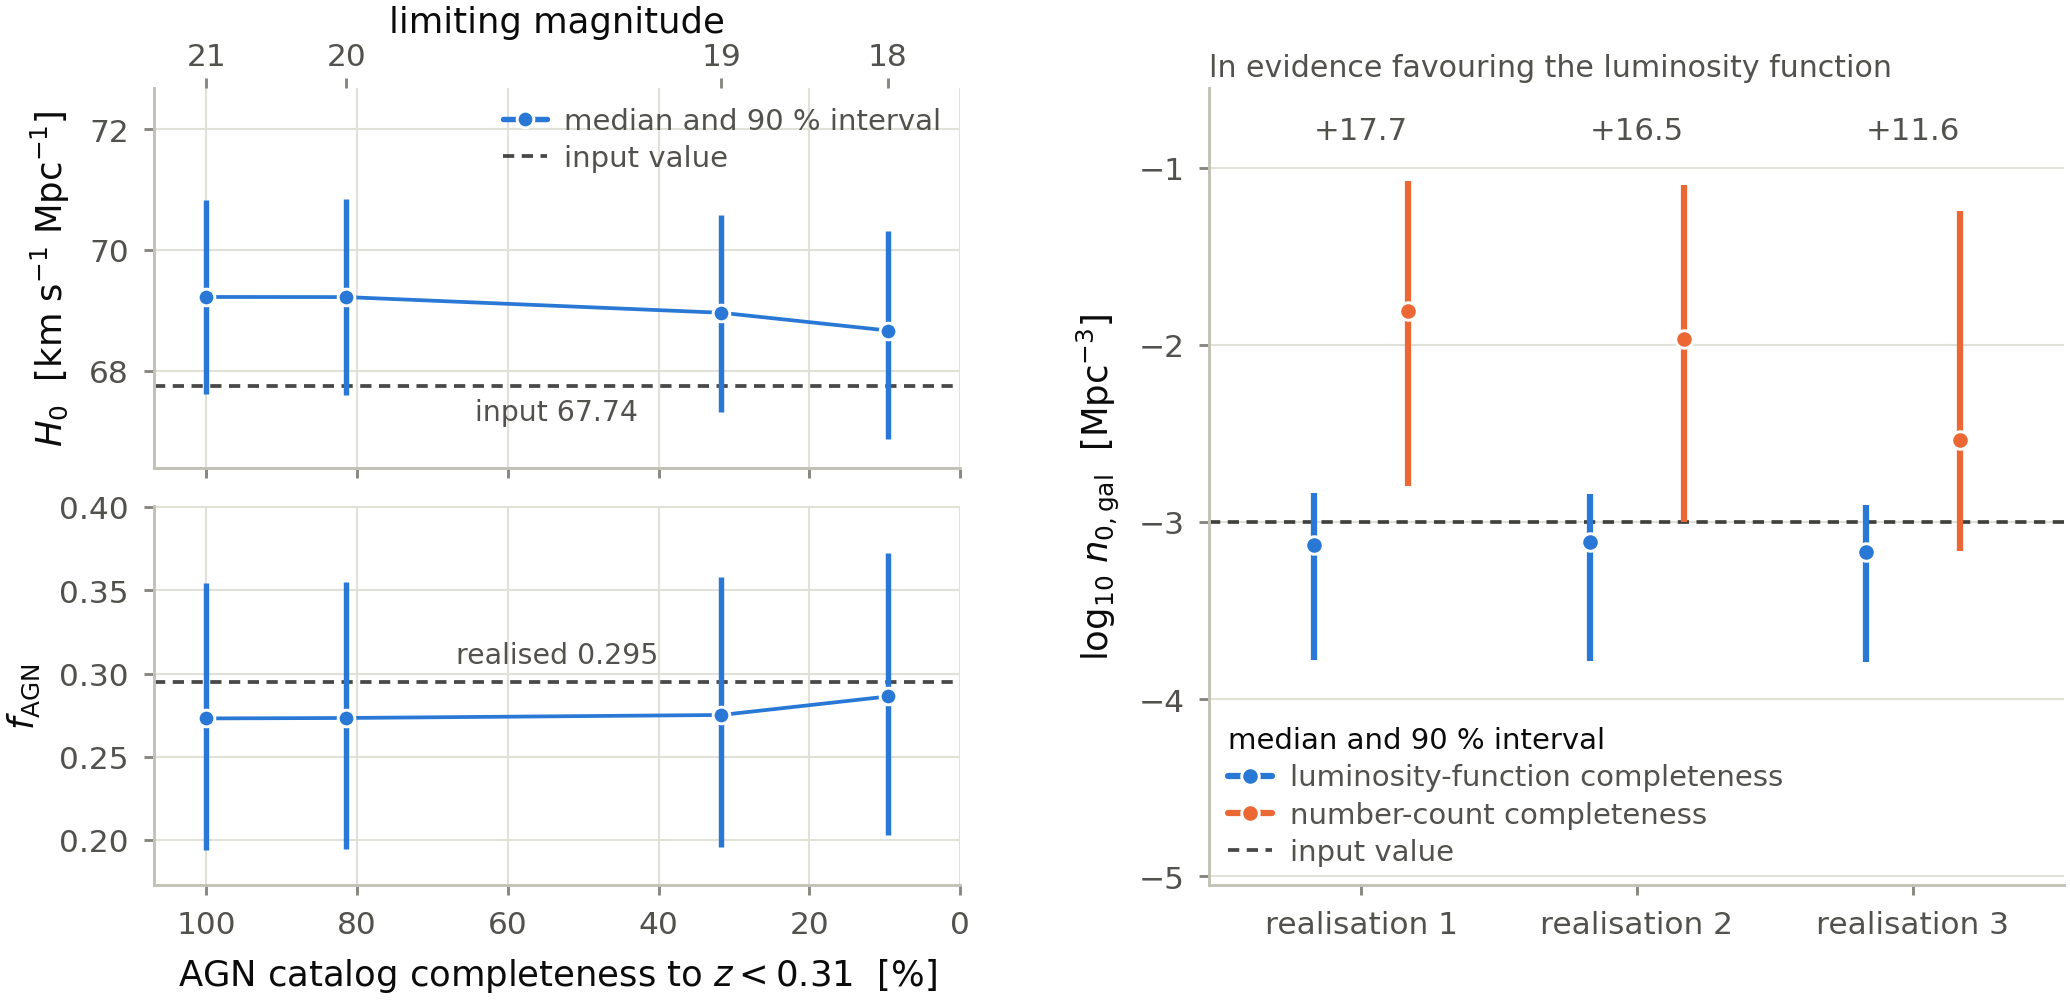
\includegraphics[width=\textwidth]{figures/fig_incomplete.pdf}
\caption{The joint measurement on flux-limited catalogs. Left: \Hz\ (upper)
and \fagn\ (lower) against the AGN catalog's completeness within the volume
the events occupy, with the corresponding magnitude limit on the upper
axis, the completeness of each catalog computed from its magnitude limit
and its luminosity function, and both number densities held at their input
values, on the reference realisation of the simulated universe. Points and
bars are medians with 90\% intervals; dashed lines mark the input expansion
rate and the realised hosted fraction. Right: the galaxy number density
recovered with both densities free at the shallowest limit, on three
independent realisations, under luminosity-function completeness and under
number-count completeness; bars are 90\% intervals, the dashed line is the
input value, and each annotation is that realisation's ln evidence
favouring the luminosity function. The number-count medians overstate the
density by \PixelAnchorBiasMinDex\ to \PixelAnchorBiasMaxDex~dex; the
luminosity-function intervals contain the input value in all three
realisations, the number-count intervals in one.
\label{fig:incomplete}}
\end{figure*}

A flux-limited survey removes hosts, and the mixture must complete both
catalogs to keep its weight meaningful. Repeating the joint fit on the
flux-limited catalogs of \S\ref{sec:data:survey}, with each catalog's
completeness computed from its magnitude limit and its luminosity function
(\S\ref{sec:methods:completion}) and both number densities held at their
input values, preserves the measurement at every depth on the reference
realisation (Figure~\ref{fig:incomplete}): the input \Hz\ lies inside the
90\% interval at the three deeper limits and the 68\% at the shallowest,
and \fagn\ holds the realised fraction inside the 68\% at all four. At the
shallowest limit, where \CompMEighteen\ per cent of hosts remain
catalogued, we find $\Hz = \HzeroIncomplete$~\kmsmpc\ and
$\fagn = \FagnIncomplete$, the \fagn\ interval essentially unchanged from
the complete catalogs (a factor of \FagnWidthRatio).

Anchoring the densities is the strongest assumption the completion makes,
and it can be dropped. Freeing both $n_{0,k}$ under flat priors at the
shallowest limit returns the galaxy density to within
\GalDensityFreeOffsetDex~dex of the input value, inside the 68\% interval
($\log_{10} n_0 = \GalDensityFree$); the widening falls almost entirely on
the fraction, whose interval grows by a factor of \FagnFreeWidthRatio\
($\fagn = \FagnFree$). In all three realisations the free-density \fagn\
median lies \FagnFreeOffsetMin\ to \FagnFreeOffsetMax\ above the reference
fraction, each inside its own 68\% interval; three realisations do not
resolve whether that offset is systematic. The dependence on the assumed
density is continuous rather than a cliff; at fixed depth, a one-dex error
in the assumed AGN density moves \fagn\ by \FagnDensitySlope. The fraction
is only as well determined as the AGN number density.

The completeness itself can be estimated two ways, from the survey's
selection or from the observed counts (\S\ref{sec:methods:completion}), and
the data distinguish them. Repeated on \NSeedsIncomplete\ independent
realisations at the shallowest limit with both densities free,
number-count completeness places the galaxy density \PixelAnchorBiasMinDex\
to \PixelAnchorBiasMaxDex~dex above the input, luminosity-function
completeness holds it within \GalAnchorOffsetMaxDex~dex with the input
inside the 68\% interval in every realisation, and the data prefer
luminosity-function completeness by \SeedLnBFmin\ to \SeedLnBFmax\
$e$-folds of evidence (Figure~\ref{fig:incomplete}, right).

\Hz\ is the robust parameter of the pair, within a stated limit. While the
catalogs remain at least \CompMTwenty\ per cent complete, a factor-of-two
error in the assumed AGN density moves \Hz\ by
\HzDensityShiftFactorTwoDeep~\kmsmpc; at \CompMEighteen\ per cent
completeness the same error displaces it by
\HzDensityShiftFactorTwo~\kmsmpc\ (\HzDensitySlopeShallow~\kmsmpc\ per
dex), half the complete-catalog interval of \HzeroJointWidth~\kmsmpc. A survey working at such depths must know the AGN
density it assumes, for the expansion rate and not only for the fraction.

\section{Validation}
\label{sec:validation}

\begin{figure*}[t]
\centering
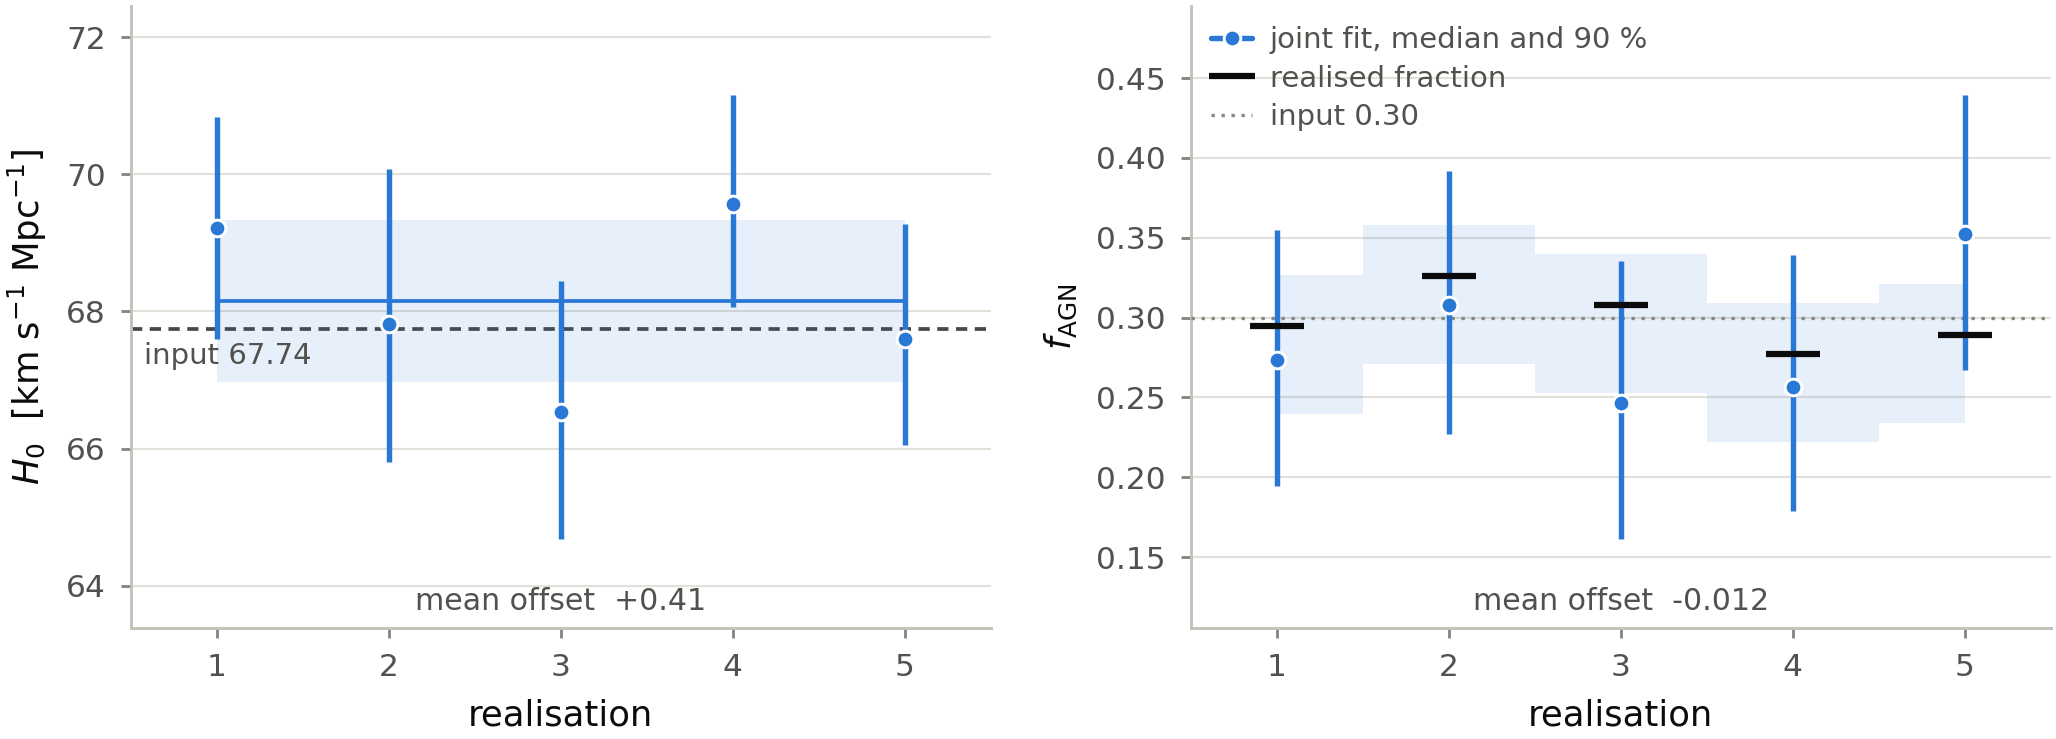
\includegraphics[width=\textwidth]{figures/fig_closure.pdf}
\caption{The joint measurement repeated on \ClosureNseeds\ independent
realisations of the simulated universe, each with its own density field,
catalogs and \EvNobs\ events. Points and bars are per-realisation medians
with 90\% intervals; the shaded band is the 90\% interval on the mean offset
over the \ClosureNseeds\ realisations. Left: \Hz\ against the input value
(mean offset $\ClosureHzero$~\kmsmpc). Right: \fagn\ against each
realisation's own realised hosted fraction (black ticks; mean offset
$\ClosureFagnReal$); the band steps because the reference differs per
realisation, and the dotted line is the input probability \FagnTruthPlanted.
The mean offsets are consistent with zero.
\label{fig:closure}}
\end{figure*}

The measurement of \S\ref{sec:results:joint} rests on one realisation of
every random step in \S\ref{sec:data}: the density field, the catalogs
drawn from it, the hosts, the measurements, and the injection sets. We
repeat the entire construction \ClosureNseeds\ times with independent draws
and repeat the joint measurement on each (Figure~\ref{fig:closure}). The
mean offsets are consistent with zero.

The mean offset of \Hz\ from the input value is $\ClosureHzero$~\kmsmpc,
and the mean offset of \fagn\ from each realisation's own hosted fraction is
$\ClosureFagnReal$ ($\ClosureFagnPlanted$ against the input probability).
The input values fall inside the 68\% intervals in
\ClosureHzeroInSixtyEight\ of \ClosureNseeds\ realisations for \Hz\ and
\ClosureFagnInSixtyEight\ for \fagn, and inside the 90\% intervals in
\ClosureHzeroInNinety\ and \ClosureFagnInNinety, consistent with the
nominal rates for \ClosureNseeds\ draws. The realisation-to-realisation
scatter of the \Hz\ medians is \ClosureScatterHzeroRatio\ times the mean
quoted half-width (\ClosureScatterFagnRatio\ for \fagn), so the quoted
intervals are honest to the precision \ClosureNseeds\ realisations can test.
The matched-host controls of \S\ref{sec:results} also recover across
realisations, with mean offsets of $\CtrlGalMean$~\kmsmpc\ (galaxies; the
input value inside the 68\% interval in \CtrlGalInSixtyEight\ of
\CtrlNseeds\ realisations and inside the 90\% in \CtrlGalInNinety) and
$\CtrlAgnMean$~\kmsmpc\ (AGN; \CtrlAgnInSixtyEight\ of \CtrlNseeds\ at 68\%
and \CtrlAgnInNinety\ at 90\%). The correlation between the two parameters
stays small across realisations, $\rho = \JointRhoMean$.

\PureNseeds\ realisations measure not only whether the single-catalog
analyses of \S\ref{sec:results:single} recover the input value but how wide
their intervals should be, and the two tracers answer differently. The
realisation-to-realisation scatter of the galaxy medians is \EnsGalRatio\
times the mean quoted 68\% half-width, so the galaxy interval is the size it
claims to be. The AGN interval is not. Its scatter is \EnsAgnRatio\ times the
quoted half-width, and its coverage sits below the diagonal across the whole
range of credible levels in Figure~\ref{fig:pure}. The matched-host controls
show the same contrast over \EnsCtrlNseeds\ realisations, \EnsCtrlGalRatio\
for galaxies against \EnsCtrlAgnRatio\ for AGN, and those controls divide one
event set by host type rather than drawing a new one, so the deficit follows
the sparse catalog rather than the choice of events. We read it as sample
variance of the sparse catalog itself, which a fit conditioned on the catalog
it was given cannot see; the realisations redraw catalogs and events together,
so they do not separate that from variance in which events are detected.
Inflating each tracer's half-width by its own measured factor moves the sparse
catalog's advantage at equal event count from $\PureWidthRatioPerSeed$ to
\EnsWidthRatioCorrected\ in the ratio of half-widths. The sparse catalog still
carries more information per event that belongs to it; what moves is how much.

The free-density flux-limited fit replicates as well. Repeated on
\NSeedsIncomplete\ independent
realisations at the shallowest limit, it stays within
\GalAnchorOffsetMaxDex~dex of the input galaxy
density, with the input value inside the 68\% interval in every realisation.
In each the data prefer the luminosity-function completeness over the
number-count completeness by at least \SeedLnBFmin\ $e$-folds
(\S\ref{sec:results:incomplete}).

With \Hz\ held at its input value, the events as observed give
$\fagn = \FagnRecord$ (68\% interval \FagnRecordCi), and permuting the
observed sky positions among the events, so that every event keeps its
distance and its localisation area but no longer points at its own host,
collapses the recovered fraction to \FagnNull\ (\FagnNullCi). The
observed-sky value lies far outside the permuted data's 90\% range,
\FagnNullCiNinety, so host association, not the catalogs' global structure,
carries the measurement.

The mixture likelihood contains both single-catalog analyses as its
endpoints: at $\fagn = 0$ and $\fagn = 1$ its likelihood and its selection
integral reduce to the single-catalog ones, and the evaluated posteriors
reproduce the measurements of \S\ref{sec:results:single} to machine
precision. An injection set drawn independently of the
catalogs, from the source population and the comoving volume alone,
reproduces the joint medians: $\Hz = \HzeroJointCross$ against
\HzeroJointMedian~\kmsmpc\ on a 68\% width of \HzeroJointWidth, and
$\fagn = \FagnJointCross$ against \FagnJointMedian\ on a width of
\FagnJointWidth. Finally, the detectable fraction $\mu(\Lambda)$ of
Equation~(\ref{eq:mu}) is a Monte Carlo estimate, and its error moves every
event coherently rather than averaging away. The error of the mixture's own
term is not measured directly, but its $\fagn = 0$ and $\fagn = 1$ limits
bracket it between \SelMcJointLo\ and \SelMcJointHi~\kmsmpc\ per
realisation; carried onto the mean over the \ClosureNseeds\ realisations it
is at most half that mean's standard error.

\section{Discussion}
\label{sec:discussion}

The measurement establishes that a second, much sparser host catalog is not
merely a weaker substitute for a galaxy catalog in a dark standard siren
analysis: because the two catalogs trace the same structure with different
number density and different bias, the fraction of mergers hosted by each is a
parameter of the same likelihood that measures the expansion rate, and it is
measured on the same events. A branching ratio between formation channels
\citep{FordMcKernan2022} therefore becomes accessible to the data that already
constrain \Hz, with no electromagnetic counterpart and no host identification.

What identifies \fagn\ sets what the result does and does not depend on. The
two catalogs differ in
their comoving number density by a factor \DensityRatio\ and in their linear
bias by a factor \BiasRatioMeas, and both differences enter the line-of-sight
redshift prior through Equation~(\ref{eq:pcat}) once each catalog's sky
weighting is normalised over the survey as a whole. \fagn\ is therefore
identified by the contrast between the two priors, that is, by how many
catalogued hosts of each kind lie along a line of sight and how strongly each
kind concentrates into the same structures. It is not identified by any
difference in the mass or spin distributions of the mergers themselves, which
are identical between the two components by construction, nor in the smooth
redshift law both populations share.

Three inputs carry the measurement, and each names a requirement for a real
analysis. The first is the AGN number density: \fagn\ is a weight between two
completed priors, so the analysis must know how many AGN it cannot see; an
error in \nzagn\ must move \fagn\ with it, an expectation the flux-limited
analyses of \S\ref{sec:results:incomplete} confirm: a one-dex error in the
assumed density moves \fagn\ by \FagnDensitySlope. Hard X-ray census work
already fixes the space density of survey-defined AGN classes at the
ten-per-cent level \citep{Ananna2022}; the harder question, which
population-synthesis work puts at a factor of a few, is which AGN class hosts
the mergers \citep{McKernan2018, FordMcKernan2022}. The second is
completeness: a real survey is flux limited, and the analyses of
\S\ref{sec:results:incomplete} measure the penalty on this same simulated
universe. It falls on the fraction, not the expansion rate: the input \Hz\
lies inside the 90\% interval at the three deeper limits and the 68\% at
the shallowest, and a factor-of-two error in the assumed AGN density moves
it by \HzDensityShiftFactorTwoDeep~\kmsmpc\ while the catalogs remain more
than \CompMTwenty\ per cent complete, by \HzDensityShiftFactorTwo~\kmsmpc\
at \CompMEighteen\ per cent. The requirement is on each catalog's absolute
density rather than on the two surveys reaching comparable depth: moving
the galaxy and AGN magnitude limits independently, over
\RelCompletenessSpanDex~dex in the ratio of the two completenesses, changes
\fagn\ by \FagnRelSpan\ and \Hz\ by \HzeroRelSpan~\kmsmpc\ from end to end,
neither resolved against a single fit's statistical error. The
completeness itself must come from the survey's selection, with a
luminosity function known independently of the survey's own photometric
scatter: number-count completeness misplaces the recovered galaxy density
by up to \PixelAnchorBiasMaxDex~dex, and the data disfavour it by
\SeedLnBFmin\ to \SeedLnBFmax\ $e$-folds of evidence. The third is the
source population, held at its input values throughout; in a real analysis
the mass distribution is uncertain jointly with the cosmology
\citep{GWTC3Cosmo2023}, and we have not tested the mixture against that
freedom.

The measurement itself asks for nothing exotic: a galaxy catalog, an AGN
catalog over the same footprint with a defensible number density, and the
dark-siren machinery already in production use. The mixture weight it returns
is the branching ratio that AGN-channel population studies parameterise from
the mass and spin side \citep{FordMcKernan2022, TagawaHaimanKocsis2020}. A
host-statistics measurement of the same number would be independent of both,
and it arrives at no cost to the expansion rate: the same fit that measures
\fagn\ is also the sharpest \Hz\ of the analyses that use every event. As
the detected sample grows toward thousands of events, and once the mixture
is fitted with the mass distribution free rather than fixed, the question
stops being whether the AGN-hosted fraction can be measured and becomes
which catalogs to measure it against.


\appendix
\section{Each catalog at equal event counts}
\label{app:pure}

The single-catalog analyses of \S\ref{sec:results:single} confound two things:
what a catalog's redshift prior is worth per event, and the cost of the events
it does not host. To separate them, we drew two further sets of
\PureNevents\ detected events for each realisation of the simulated universe,
one with every host a galaxy and one with every host an AGN, each with
independent measurement noise, and analysed each set against its own
catalog alone, exactly as in \S\ref{sec:results:single} but with nothing
misassigned.

\begin{figure*}[t]
\centering
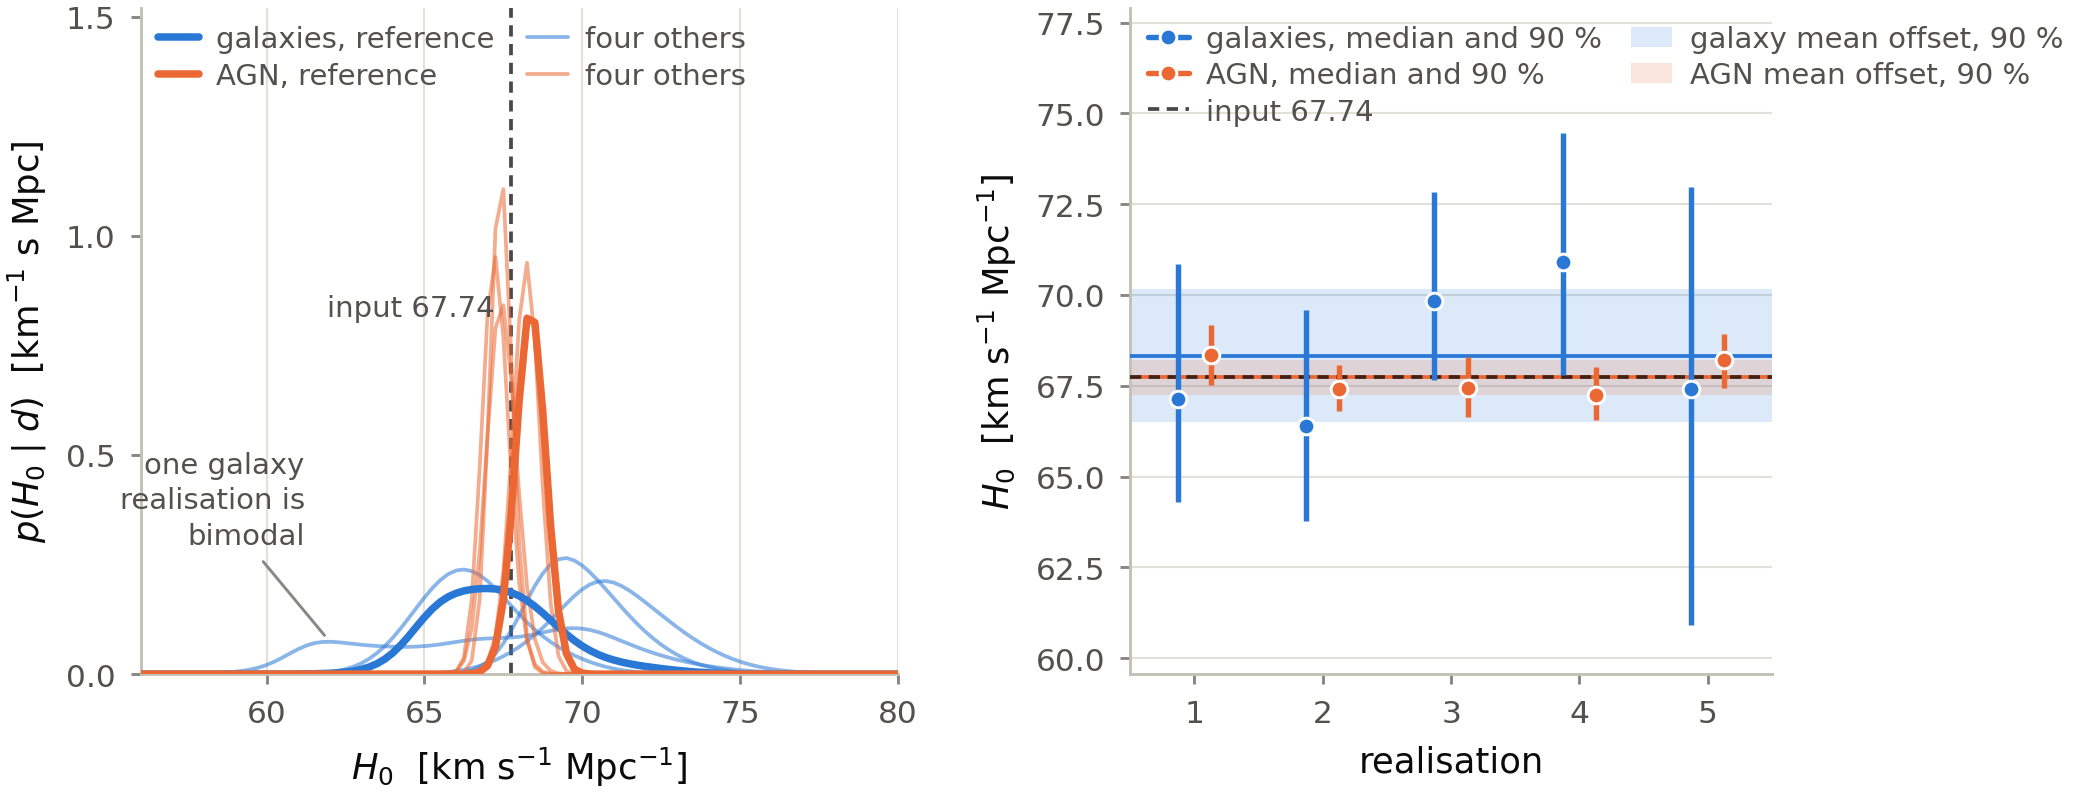
\includegraphics[width=\textwidth]{figures/fig_pure_tracer.pdf}
\caption{What each catalog delivers on events it actually hosts. For every
realisation of the simulated universe, two further sets of \PureNevents\
detected events were drawn on the same catalogs, every host a galaxy
(blue) or every host an AGN (orange), and each set analysed against its
own catalog alone, with \Hz\ the only free parameter. Left: the ten
normalised posterior densities $p(\Hz \mid d)$, in units of
km$^{-1}$\,s\,Mpc, on one shared density axis with no rescaling, and the
input value dashed; the reference realisation is drawn at full strength and
the other four lighter in the same hue, and the \Hz\ axis spans
$[56, 80]$~\kmsmpc, outside which every curve holds less than $10^{-4}$ of
its mass. The bimodal galaxy realisation
(realisation \PureBimodalSeed, second mode at \PureBimodalModeLo~\kmsmpc\ at
\PureBimodalHeight\ of the primary mode at \PureBimodalModeHi) is drawn as it
is. Right: the same ten
measurements as medians with 68\% intervals against the same input line,
the two tracers offset slightly from each other at each realisation for
legibility, with each tracer's five-realisation mean offset and its standard
error as line and band. At equal event count, the catalog one hundred times
sparser is a factor of \PureWidthRatio\ sharper.
\label{fig:pure}}
\end{figure*}

Both catalogs recover the input value. Over the \PureNseeds\ realisations the
mean offsets are $\PureAgnOffset$~\kmsmpc\ from the AGN sets and
$\PureGalOffset$ from the galaxy sets, with the input inside the 90\%
intervals in \PureAgnInNinety\ and \PureGalInNinety\ of \PureNseeds\
realisations (Figure~\ref{fig:pure}); the medians agree with those from the
independent cross-check injection set to at most \PureLaneMaxAgn\ of the
corresponding half-width across all twenty analyses. One galaxy realisation
is bimodal, with a second mode at \PureBimodalModeLo~\kmsmpc\ standing at
\PureBimodalHeight\ of the primary mode at \PureBimodalModeHi, and that
second mode is what widens the galaxy
mean offset's standard error; the cross-check on the same events is
unimodal.

What separates the tracers is the width. At the same event count the AGN
catalog measures the expansion rate with a mean 68\% half-width of
\PureAgnHalfWidth~\kmsmpc\ against the galaxy catalog's \PureGalHalfWidth,
a factor of \PureWidthRatio, stable across realisations (per-realisation
ratio $\PureWidthRatioPerSeed$). A catalog one hundred times sparser is not a
weaker version of the same prior: per event that actually belongs to it, it
is several times stronger, because each event's line of sight holds a handful
of candidate hosts rather than a smooth crowd. This is the per-event
information behind the reading of \S\ref{sec:results:joint}, that the joint
fit gains by letting the AGN-hosted events be anchored by the sparse
catalog.


\bibliographystyle{aasjournal}
\bibliography{references}

\end{document}
